\documentclass[11pt,a4paper]{article}
\usepackage[T1]{fontenc}
\usepackage{lmodern}
\usepackage{a4wide}
\usepackage[dvips]{graphicx}
\usepackage{float}

\usepackage[
pdfauthor={ACE Projekt Team},
pdftitle={Evaluation Algorithms},
pdfcreator={pdftex},
]{hyperref}

\usepackage{sectsty}
\allsectionsfont{\sffamily}

\usepackage{fancyheadings} 
\pagestyle{fancy} 
\lhead{\textsf{\textbf{ACE} \\ \small{a collaborative editor}}}
\chead{}
\rhead{
\parbox[c]{3cm}{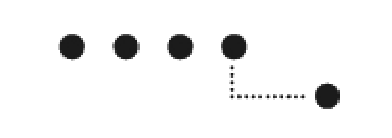
\includegraphics[height=0.875cm,width=3cm]{../../images/logo_BFH.eps}}
\parbox[c]{2.2cm}
{\tiny{\textsf{Berner Fachhochschule \\
Hochschule f�r \\
Technik und Informatik}}}}
\lfoot{}
\cfoot{\textsf{\thepage}}
\rfoot{}
\setlength{\headrulewidth}{0.6pt}
\setlength{\footrulewidth}{0.6pt}
\setlength{\topmargin}{-50pt}
\addtolength{\headheight}{50pt}

\usepackage{colortbl}

\newcommand{\headercol}[2]{\multicolumn{1}{|>{\bfseries\columncolor[gray]{0.82}}p{#1}|}{\textsf{#2}}}
\newcommand{\ace}[0]{\emph{ACE }}



\begin{document}
\setlength{\parindent}{0pt}

\newtheorem{defn}{Definition}

\bibliographystyle{plain}

\begin{titlepage}
\thispagestyle{empty}
  
\includegraphics[height=1.5in]{../images/pix.eps}

  \begin{center}

    {\fontsize{40}{45} \textbf{\textsf{ACE}}} \\
    \textsf{a collaborative editor} \\
        
    \vspace{36pt}
        
    {\huge{\textbf{\textsf{}}}} \\

    \vspace{36pt}

	\textsf{Berne University of Applied Sciences} \\
    \textsf{School of Engineering and Information Technology} \\
    
  \end{center}

  \vfill
  
  \begin{tabular}{ll}
   \hline

   \\

   \multicolumn{1}{>{\bfseries}p{1.5in}}{\textsf{Date:}} &
   \multicolumn{1}{>{}p{4.3in}}{\textsf{08.11.2005}}          \\
   
   \\
   
   \multicolumn{1}{>{\bfseries}p{1.5in}}{\textsf{Version:}}     &   
   \multicolumn{1}{>{}p{4.3in}}{\textsf{0.1}}                 \\

   \\
   
   \multicolumn{1}{>{\bfseries}p{1.5in}}{\textsf{Projectteam:}}                 &
   \multicolumn{1}{>{}p{4.3in}}{\textsf{Mark Bigler (biglm2@hta-bi.bfh.ch)}}  \\
   \multicolumn{1}{>{\bfseries}p{1.5in}}{}                                      &
   \multicolumn{1}{>{}p{4.3in}}{\textsf{Simon Raess (rasss@hta-bi.bfh.ch)}}    \\
   \multicolumn{1}{>{\bfseries}p{1.5in}}{}                                      &
   \multicolumn{1}{>{}p{4.3in}}{\textsf{Lukas Zbinden (zbinl@hta-bi.bfh.ch)}} \\   
   
   \\
   
   \multicolumn{1}{>{\bfseries}p{1.5in}}{\textsf{Receivers:}}                       &
   \multicolumn{1}{>{}p{4.3in}}{\textsf{Jean-Paul Dubois (doj@hta-bi.bfh.ch)}}       \\
   \multicolumn{1}{>{\bfseries}p{1.5in}}{}                                          &
   \multicolumn{1}{>{}p{4.3in}}{\textsf{Claude Fuhrer (frc@hta-bi.bfh.ch)}}       \\

   \\
   
   \multicolumn{1}{>{\bfseries}p{1.5in}}{\textsf{Location:}}               &   
   \multicolumn{1}{>{}p{4.3in}}{\textsf{Subversion Repository}} \\

   \\  
   
   \hline
  \end{tabular}

\end{titlepage}

\newpage

\tableofcontents
\newpage
\listoftables
\listoffigures
\newpage



\section{Introduction}
The purpose of this report is to show usability requirements for a user-friendly collaborative editor. The most useful functions will be discussed in the following chapters. There are also prototypes for some of these functions to ensure the feasibility with \emph{Java} text components.

\section{Usability}
Basically each user must be distinguishable from all the other users. To do that with different colors is probably one of the best solution. For example the red user has a dark red colored cursor, a light red color to highlight the text he changed and a red border around the text he selected. The users are listed with their colors in a separate window, so all participants can quite easily see which part in the multi-colored text document belongs to which user. It is important that each user is aware of other user's actions in order to avoid possible conflicts, for example two users correcting the same spelling mistake. See \cite{usability} for more information about usability in groupware systems.

\subsection{Main View}
The main view is the users workspace where he can change the document or observe the other users. Important is to keep the main view as simple as possible. This means that it should not be overloaded with a lot of buttons, status labels, etc. because new users will loose their orientation.
\begin{figure}[H]
\centering
\frame{
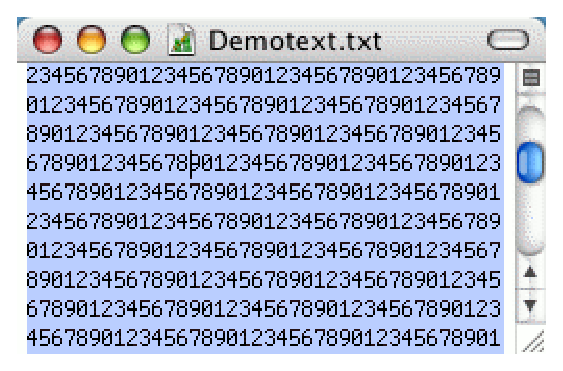
\includegraphics[height=3cm,width=5cm]{../../images/gui/gui_main_view.eps}
}
\caption{Main View}
\end{figure}

\subsection{Multiple Cursors and Telepointers}
Displaying the cursors of the other participants is a very useful feature for observing their actions. These additional cursors must be clearly distinguishable and assigned to a user. Coloring all cursors with the user color (e.g. the green users cursor is painted in dark green) will be the most comfortable way to realize that. Moreover, to even further help users distinguish these other cursors from their own cursor, they should have another form than the standard cursor.

As described above for multiple cursors, it will be user friendly to display the content of the document in different colors too. In this way all participants know which part of the document originate from which user.
\begin{figure}[H]
 \centering
 \frame{
 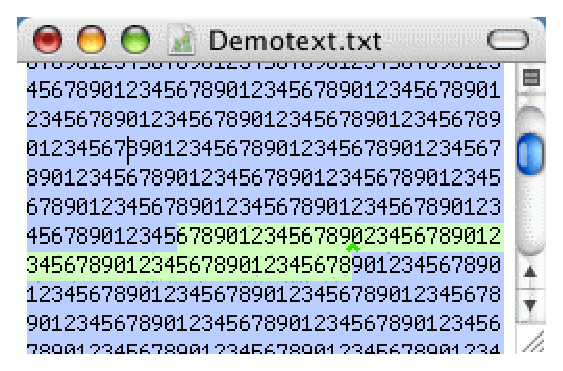
\includegraphics[height=3cm,width=5cm]{../../images/gui/gui_hlight_and_cursor.eps}
 }
 \caption{Multiple Cursors and Highlighted Text}
\end{figure}
The other users mouse cursors are called telepointers. With these telepointers it is possible to point to something in the document. It should be possible to activate/deactivate this telepointers because a lot of different cursors and telepointers can be confusing for the users.
\begin{figure}[H]
\centering
\frame{
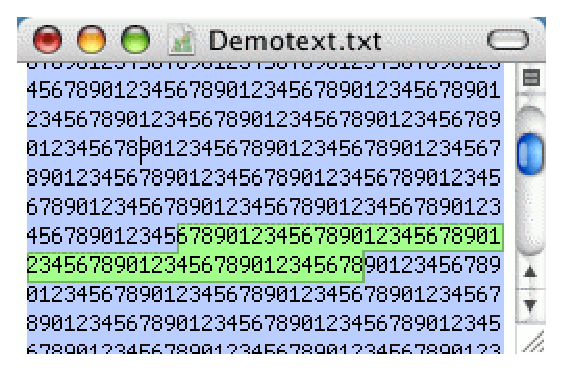
\includegraphics[height=3cm,width=5cm]{../../images/gui/gui_selection.eps}
}
\caption{Text-selection}
\label{Text-selection}
\end{figure}
The picture \ref{Text-selection} shows a possibility to represent selected text of another participant (in this case from the participant associated with the green color).

\subsection{Multi-user Scrollbar}
The aim of multi-user scrollbars is to give a coarse overview of all cursor positions in the document. A user will see his own position by a normal scrollbar and in addition a little colored symbol for the position of each other user.
\begin{figure}[H]
\centering
\frame{
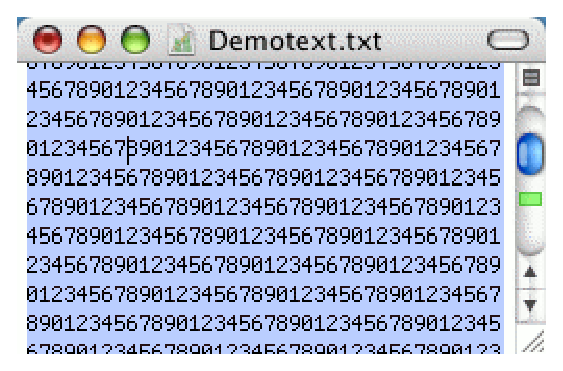
\includegraphics[height=3cm,width=5cm]{../../images/gui/gui_scrollbar.eps}
}
\caption{Multi-user Scrollbar}
\end{figure}

\subsection{Teleport and Split View}
Two similar ways to display the other users view exist. First there is the Teleport function which allows the user to see temporarily the main view of another user. To observe other users for a longer time, a split view should be provided.

\subsection{Document and User Handling}
In a collaborative application, it must be possible to publish a document, so other users can join the editing. Other users will discover these documents and can opt to join. The publisher allows or denies access based on access rights he determines. The process of publishing and joining documents as well as assigning access rights should be as seamless as possible in order to provide a great user experience.

A possible solution could be based on drag \& drop. Browsing for available documents can be realized by a little new window representing all active users in a tree view. Assigned to each user in the tree are the documents published by this user. By double clicking on such a document one can ask permission to join it. Of course the users can assign access rights to each shared document. This can be realized by a list docked to each open document where the owner of the document can drag \& drop requesting users from the category "Awaiting" to the category "Read/Write" or "Read/Only".


\section{Requirements}
In this section, we describe the basic requirements for the graphical user interface of a collaborative text editor.

\subsection{Intercept User Input}
Because all user inputs must be first processed by the synchronization algorithm, the text component must be able to catch all the keyboard inputs.

\subsection{Awareness Information}
As seen in the last section, it is important in a collaborative application that users are aware of other user's actions. Important awareness information includes telecursors and multi-user scrollbars. Less important, but still useful , are telepointers.

It would be helpful if one can follow other users actions. For this reason, a split view should be provided that follows the other users cursor.

\subsection{Discover Published Documents}
A user should have a straightforward way to discover other published documents. These documents should be displayed in user interface component and allow the user to join them.

\subsection{Publish Documents}
A user should have the opportunity to publish a document (i.e. make it publicly available so others can join the document). The publisher of a document should have a simple way to specify the access rights for the document (e.g. read-only or full-access).


\section{Prototypes}
Prototypes are used to ensure that the requirement described above can be realized with java text components.

\subsection{CustomPaint}
\paragraph{Purpose:}
The aim of this prototype is to find out the best way to represent more than one cursor in a text component.
\paragraph{Description:}
This prototype is a little class extending \texttt{JTextPane}. The main functionality is in the overridden paint method which looks like:
\begin{verbatim}
public void paintComponent(Graphics g) {
  super.paintComponent(g);
  for each cursor to display
    get the cursor position;
    get the cursor color;
    draw the cursor;
}
\end{verbatim}
\paragraph{Notes:}
There is a problem with rendering cursors in other lines than the real cursor is. A simple \texttt{repaint} call at the end of the \texttt{paintComponent} method will avoid that but thats no a proper solution.



\subsection{CustomView}
\paragraph{Purpose:}
This prototype shows another way to display more than one cursor in a text component.
\paragraph{Description:}

First of all, a editor kit to set the custom view of a text component must exist. This editor kit looks like:
\begin{verbatim}
public class CustomEditorKit extends StyledEditorKit implements ViewFactory {
  public ViewFactory getViewFactory() {
    return this;
  }
  public View create(Element elem) {
    return new CustomView(elem);
  }
}
\end{verbatim}

The functionality of the paint function of the custom view is the same as in the custom paint prototype. 
\begin{verbatim}
public class CustomView extends WrappedPlainView {
  public void paint(Graphics g, Shape a) {
    super.paint(g, a);
    for each cursor to display
      get the cursor position;
      get the cursor color;
      draw the cursor;
  }
}
\end{verbatim}

To use the custom view on a text component, the following lines are necessary.
\begin{verbatim}
JTextPane textPane = new JTextPane();
textPane.setEditorKit(new CustomEditorKit());
\end{verbatim}

\paragraph{Notes:}
This is the proper solution to display custom cursors. The only resting problem at the moment is that such a cursor cannot be larger than a text line.




\subsection{CustomDocument}
\paragraph{Purpose:}
This prototype is created for finding the best way to capture the keyboard inputs from a text component.
\paragraph{Description:}
A new styled document is needed for that prototype. The important methods to override in this class are \texttt{insertString}, \texttt{remove} and \texttt{createPosition}. Furthermore there must be some additional methods like \texttt{insertXXXString}. They are necesarry because the original \texttt{insertString} method no longer will insert text into the text component.
\begin{verbatim}
public class CatchKeyboardStyledDocument extends DefaultStyledDocument {
  public void insertSynchedString(int offs, String str, AttributeSet a)
      throws BadLocationException {
    super.insertString(offs, str, a);
  }
  public void insertString(int offs, String str, AttributeSet a)
      throws BadLocationException {
    // super.insertString(offs, str, a);
    // -> removed because we want to capture the string
    //      use insertSynchedString to insert a string
    System.out.println("from JTextPane (insert): " + str);
  }
  ... other methods ...
}\end{verbatim}


Create the text component with the custom styled document:
\begin{verbatim}
JTextPane textPane = new JTextPane(new CatchKeyboardStyledDocument());
\end{verbatim}

To insert a string into the text component:
\begin{verbatim}
((CatchKeyboardStyledDocument)
   textPane.getStyledDocument()).insertSynchedString(0, txt + "\n", null);
\end{verbatim}



\newpage
\bibliography{ace}

\end{document}
